%%%%%%%%%%%%%%%%%%%%%%%%%%%%%%%%%%%%%%%%%
% University Assignment Title Page 
% LaTeX Template
% Version 1.0 (27/12/12)
%
% This template has been downloaded from:
% http://www.LaTeXTemplates.com
%
% Original author:
% WikiBooks (http://en.wikibooks.org/wiki/LaTeX/Title_Creation)
%
% License:
% CC BY-NC-SA 3.0 (http://creativecommons.org/licenses/by-nc-sa/3.0/)
% 
% Instructions for using this template:
% This title page is capable of being compiled as is. This is not useful for 
% including it in another document. To do this, you have two options: 
%
% 1) Copy/paste everything between \begin{document} and \end{document} 
% starting at \begin{titlepage} and paste this into another LaTeX file where you 
% want your title page.
% OR
% 2) Remove everything outside the \begin{titlepage} and \end{titlepage} and 
% move this file to the same directory as the LaTeX file you wish to add it to. 
% Then add \input{./title_page_1.tex} to your LaTeX file where you want your
% title page.
%
%%%%%%%%%%%%%%%%%%%%%%%%%%%%%%%%%%%%%%%%%
%\title{Title page with logo}
%----------------------------------------------------------------------------------------
%	PACKAGES AND OTHER DOCUMENT CONFIGURATIONS
%----------------------------------------------------------------------------------------

\documentclass[12pt]{article}
\usepackage[english]{babel}
\usepackage[utf8x]{inputenc}
\usepackage{amsmath}
\usepackage{graphicx}
\usepackage{subcaption}
\usepackage{float}
\usepackage[colorinlistoftodos]{todonotes}



\textheight=230truemm 
\textwidth=160truemm 
\hoffset=-10truemm \voffset=-20truemm

\begin{document}

\begin{titlepage}

\newcommand{\HRule}{\rule{\linewidth}{0.5mm}} % Defines a new command for the horizontal lines, change thickness here

\center % Center everything on the page
 
%----------------------------------------------------------------------------------------
%	HEADING SECTIONS
%----------------------------------------------------------------------------------------

\textsc{\LARGE Ukrainian Catholic University}\\[1cm] % Name of your university/college
\textsc{\Large  Faculty of Applied Sciences}\\[0.5cm] % Major heading such as course name
\textsc{\large Data Science Master Programme}\\[0.5cm] % Minor heading such as course title

%----------------------------------------------------------------------------------------
%	TITLE SECTION
%----------------------------------------------------------------------------------------
\vspace*{1cm}

\HRule \\[0.4cm]
{ \huge \bfseries Visualization of high-dimentional data using $t$-SNE algorithm}\\[10pt]
{\Large \bfseries Linear Algebra final project report}\\[0.4cm] % Title of your document
\HRule \\[1cm]
 
%----------------------------------------------------------------------------------------
%	AUTHOR SECTION
%----------------------------------------------------------------------------------------
\vspace*{1cm}

% If you don't want a supervisor, uncomment the two lines below and remove the section above
\Large \emph{Authors:}\\
Serhii \textsc{Brodiuk}\\Andrii \textsc{Yurkiv}\\[1cm] % Your name

%----------------------------------------------------------------------------------------
%	DATE SECTION
%----------------------------------------------------------------------------------------
\vspace*{1cm}
{\large 24 January 2019}\\[2cm] % Date, change the \today to a set date if you want to be precise

%----------------------------------------------------------------------------------------
%	LOGO SECTION
%----------------------------------------------------------------------------------------


\includegraphics[height=5cm]{UCU-Apps.png}\\[1cm] % Include a department/university logo - this will require the graphicx package
 
%----------------------------------------------------------------------------------------

\vfill % Fill the rest of the page with whitespace

\end{titlepage}


\begin{abstract}
In this report we describe our implementation of $t$-SNE algorithm for visualization of multidimensional data. We compare its performance and visualization capabilities with other classic visualization algorithms and discuss its strengths and weaknesses.
	
\end{abstract}

\section{Introduction}

Data visualization is one of the most important parts of applied data analysis nowadays. Without proper visualization it’s hard, or sometimes even impossible to interpret the data in the appropriate way or make reasonable inferences regarding its structure. Dealing with data sets that contain more than 3 attributes start causing problems, because standard visualization techniques does not apply to the data in 4-dimensional space. For humans, it’s even hard to perceive graphical information in 3-dimensional space, that’s why the majority of classical techniques of data visualization are restricted to two dimensions. \\

It should be noted that one of the main purposes of visualization of high-dimensional data sets is to determine clusters inside the data which may be an important basement for further data analysis.


\section{Motivation}

Modern data often contains hundreds or even thousands of features. And classical visualization approaches cannot be used to determine patterns or clusters in it. This is the reason why so many different techniques for visualization high-dimensional data have been proposed. Majority of these techniques merely provide tools to display multidimensional data in two or three-dimensional form and do not give any inferences regarding the inner structure of the data. This severely limits the applicability of those techniques to real-world data, which sometimes contain too much features to reduce them nicely.\\

Another approach to this problem lies in the field of dimensionality reduction. We can apply classical plotting methods (for example, scatter plots) for the data obtained by decreasing the dimension of the original data set. Dimensionality reduction techniques differ substantially from visualization techniques because they are aimed not to make data more visually appealing or understandable, but to preserve as much of the significant structure of the high-dimensional data as possible in its low-dimensional representation \cite{tsnearticle}.

\section{Problem setting}

The most important goal of visualization of multidimensional data is to correctly identify clusters of similar data points. This is crucial when we are working on unsupervised learning problem and need to know for sure what number of distinct clusters can our data set be divided in without losing valuable information about inner structure of our data.\\

 As we will see in this report, many classical visualization algorithms correctly identify the relationships between data points and position similar ones together. But at the same time from visualizations those algorithms provide it's hard to tell where one class of points ends and other begins (boundaries between classes are not well-defined). And while this is not a problem for small data sets, for large ones it can cause serious obstacles for correct definition of of the number and location of data clusters. \\

$t$-SNE ($t$-distributed Stochastic Neighbor Embedding) algorithm is aimed to overcome those limitations by identifying the relevant patterns using the approach in which similar objects are modeled by nearby points and dissimilar objects are modeled by distant points with high probability \cite{tsnearticle}. 

\section{Related work}

\section{Approach to Solution}

\section{Solution}

\section{Evaluation}

Since $t$-SNE is primarily visualization technique, in order to evaluate its performance and visualizational capacity we need to compare visualization produced by t-SNE with the ones obtained using other non-parametric visualization techniques for multidimensional data, such as Multidimensional scaling using SMACOF (Scaling by Majorizing a Complicated Function) algorithm, Isomap, Locally Linear Embedding, Principal Components Analysis and Laplacian Eigenmaps. PCA is not usually used for visualization, but we decided that it would be a good idea to show how the visualizations obtained from manifold learning algorithms differ from those obtained from classic dimensionality reduction technique.\\

\subsection{Data sets}

In our work we experimented with 2 different data sets: Olivetti faces data set and handwritten digits data set.\\ 

Olivetti faces dataset contains 400 $64 \times 64$ grayscale images of faces (10 images for each of 40 subjects). Those images were taken at different time with different details varying, such as face expression, lighting and facial details (absence or presence of glasses). They are labeled according to the identity of the person depicted.\\

Handwritten digits data set consists of 1797 $8 \times 8$ grayscale images of handwritten digits of 10 classes. There are nearly 180 instances per digit class in this data set.\\

\subsection{Experimental setup}

In the original $t$-SNE paper \cite{tsnearticle}, the authors use PCA to reduce dimensionality before feeding the data into algorithms that transform it into two-dimensional representation. They are doing it for the purpose of computation efficiency and it absolutely makes sense when we apply those algorithms to large data sets. But since the data sets which we use in our experiments are relatively small, preliminar dimensionality reduction doesn't make much difference in terms of computational costs in our case, so we decided to pass this step up.\\

For each of these data sets, there is information about the class of each data point. Class information is only used for visualization purposes and is not considered during calculation of the spatial coordinates of the points in two-dimensional space. We decided to visualize the whole images instead of points on scatter plots because this kind of plot is much more understandable and provides better means of evaluating how well the mapping preserves the similarities within each class and how accurately it separates one class from the other.\\

We used library utilities in order to demonstrate visualization capacity and performance of algorithms, with which we are comparing our implementation of $t$-SNE algorithm. We used \texttt{Isomap}, \texttt{LocallyLinearEmbedding}, \texttt{MDS} and \texttt{SpectralEmbedding} classes from package \texttt{sklearn.manifold} and \texttt{PCA} class from package \texttt{sklearn.decomposition}.\\

The cost function parameters we used in our experiments are listed in Table 1. Here \textit{perplexity} represents the perplexity of the conditional probability distribution induced by the Gaussian kernel and \textit{neighbors} represents the number of nearest neighbors employed in a neighborhood graph. Multidimensional scaling was performed using SMACOF algorithm with 4 initializations and 300 iterations and without any other explicit parameters. PCA uses regular library settings.\\

For each algorithm we visualized all data points present in the data set, that's why some of them look a bit crowded with too many images. 

\begin{table}[H]
	\centering
	\begin{tabular}{| l | l |}
		\hline
		Technique & Parameters \\
		\hline			
		$t$-SNE & \textit{perplexity} = 5, 1000 iterations    \\
		MDS (SMACOF) & -  \\
		Isomap & \textit{neighbors} = 5  \\
		LLE & \textit{neighbors} = 12 \\
		PCA & - \\
		Laplacian Eigenmaps & \textit{neighbors} = 12 \\
		\hline  
	\end{tabular}\\
	\caption{Cost function parameters for the experiments.}
\end{table}

\subsection{Results}



\begin{figure}
	\centering
	\begin{subfigure}[h]{0.65\textwidth}
		\centering
		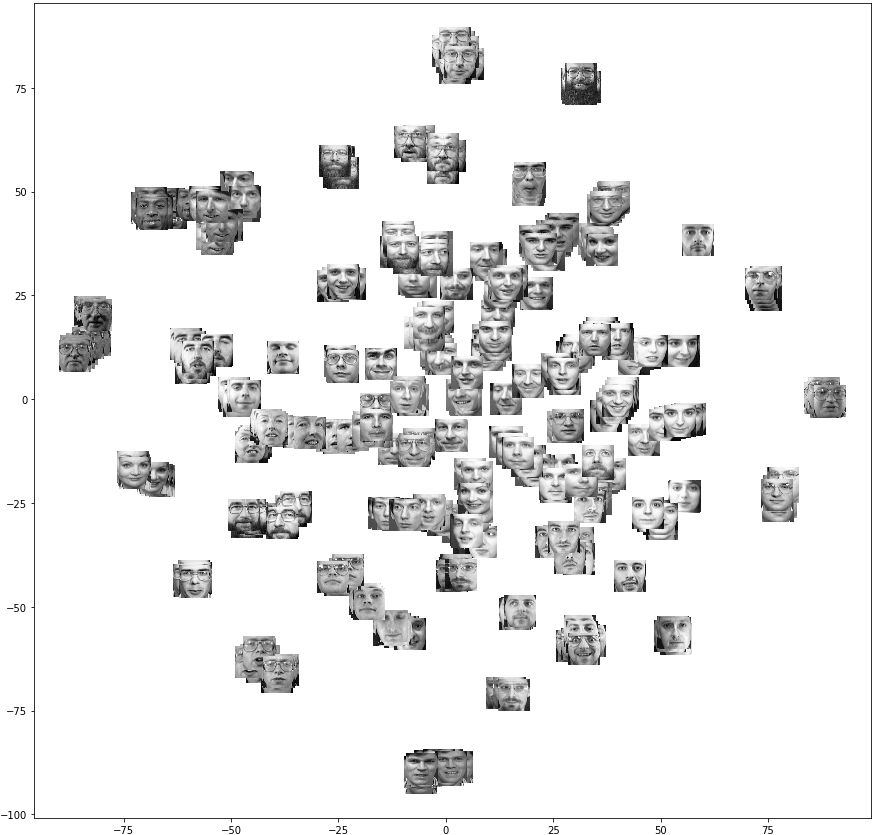
\includegraphics[width=\textwidth]{./figures/tsne_1.png}
		\caption{using $t$-SNE}
	\end{subfigure}
	
	\begin{subfigure}[h]{0.65\textwidth}
		\centering
		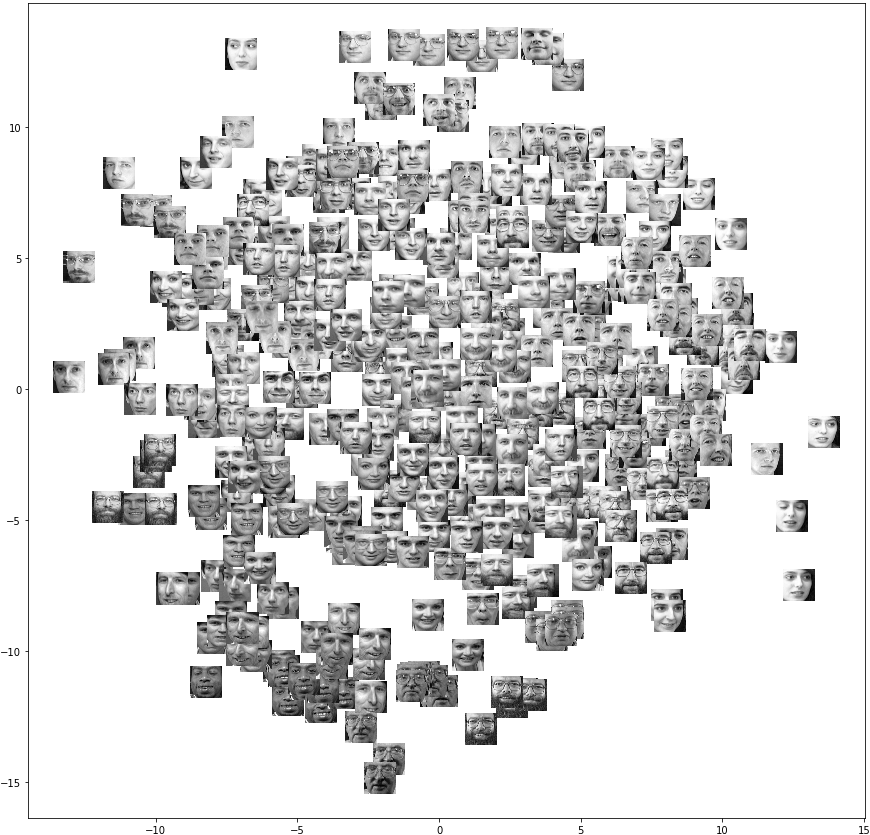
\includegraphics[width=\textwidth]{./figures/mds_1.png}
		\caption{using MDS}
	\end{subfigure}
	\caption{Visualization of Olivetti faces data set}
\end{figure}

\begin{figure}
	\centering
	\begin{subfigure}[h]{0.65\textwidth}
		\centering
		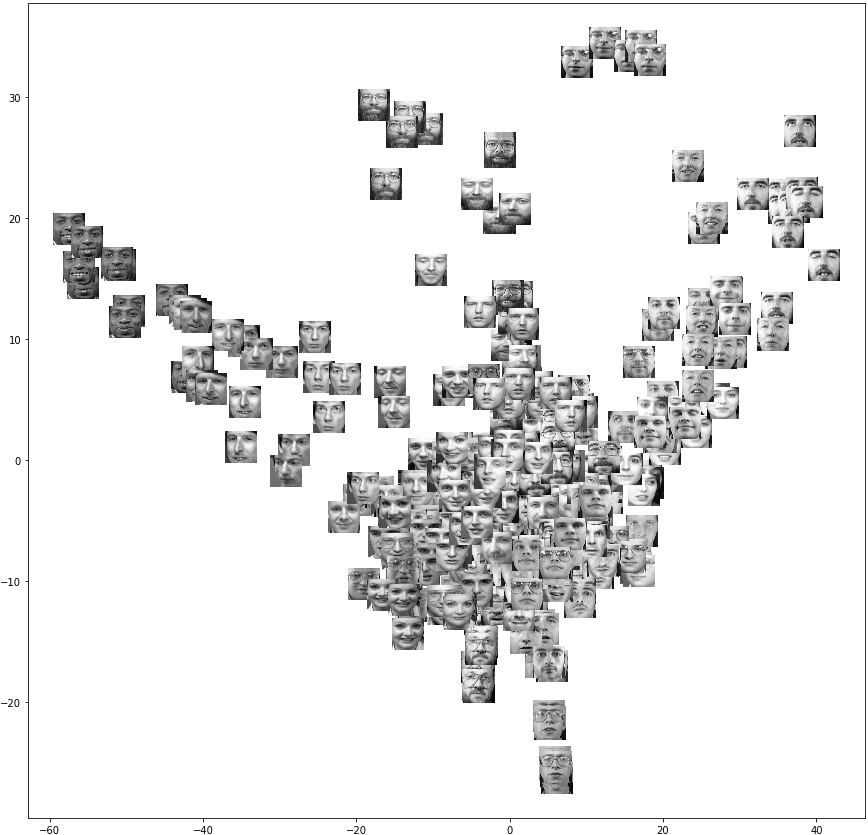
\includegraphics[width=\textwidth]{./figures/isomap_1.png}
		\caption{using Isomap}
	\end{subfigure}
	
	\begin{subfigure}[h]{0.65\textwidth}
		\centering
		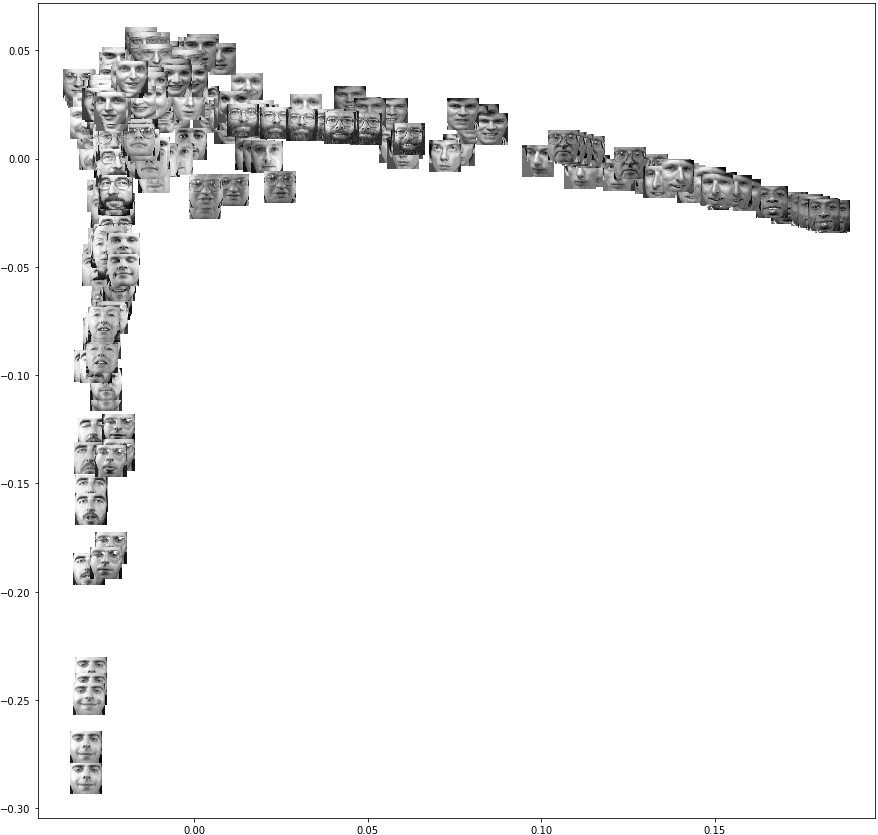
\includegraphics[width=\textwidth]{./figures/lle_1.png}
		\caption{using LLE}
	\end{subfigure}
	\caption{Visualization of Olivetti faces data set}
\end{figure}

\begin{figure}
	\centering
	\begin{subfigure}[h]{0.65\textwidth}
		\centering
		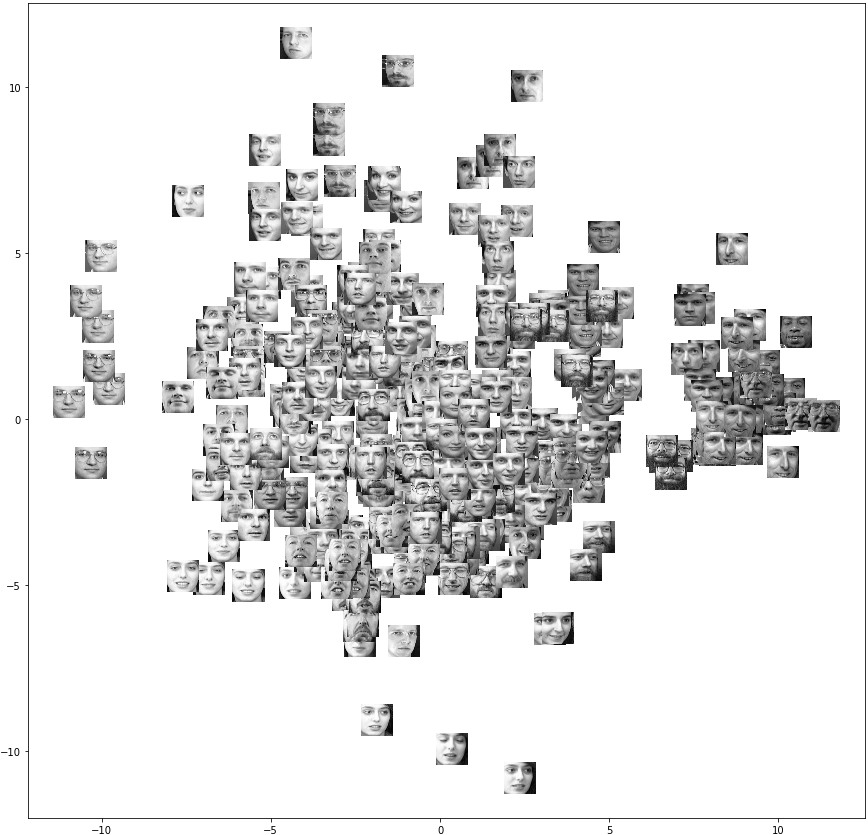
\includegraphics[width=\textwidth]{./figures/pca_1.png}
		\caption{using PCA}
	\end{subfigure}
	
	\begin{subfigure}[h]{0.65\textwidth}
		\centering
		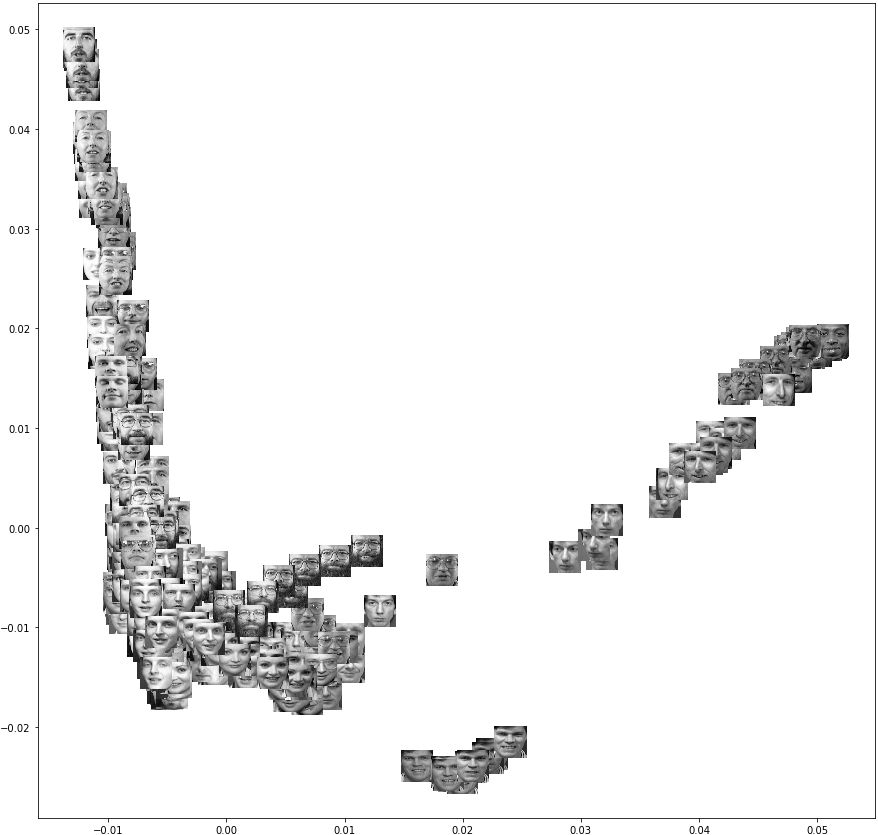
\includegraphics[width=\textwidth]{./figures/lap_1.png}
		\caption{using Laplacian Eigenmaps}
	\end{subfigure}
	\caption{Visualization of Olivetti faces data set}
\end{figure}

\begin{figure}
	\centering
	\begin{subfigure}[b]{0.4\textwidth}
		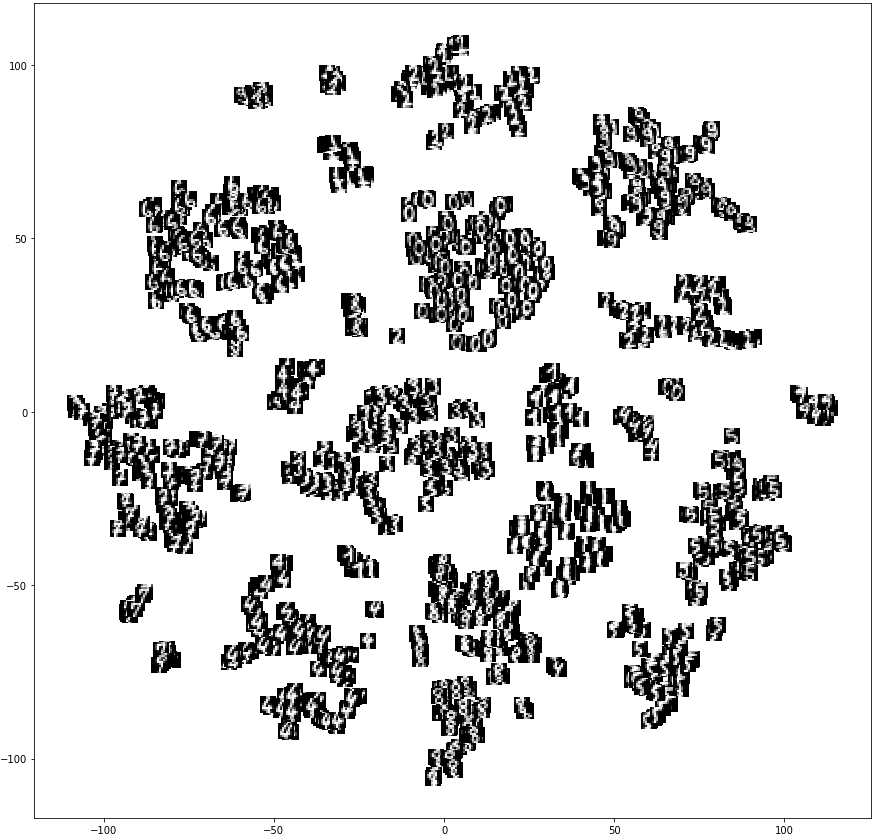
\includegraphics[width=\textwidth]{./figures/tsne_2.png}
		\caption{using $t$-SNE}
	\end{subfigure}
	~
	\begin{subfigure}[b]{0.4\textwidth}
		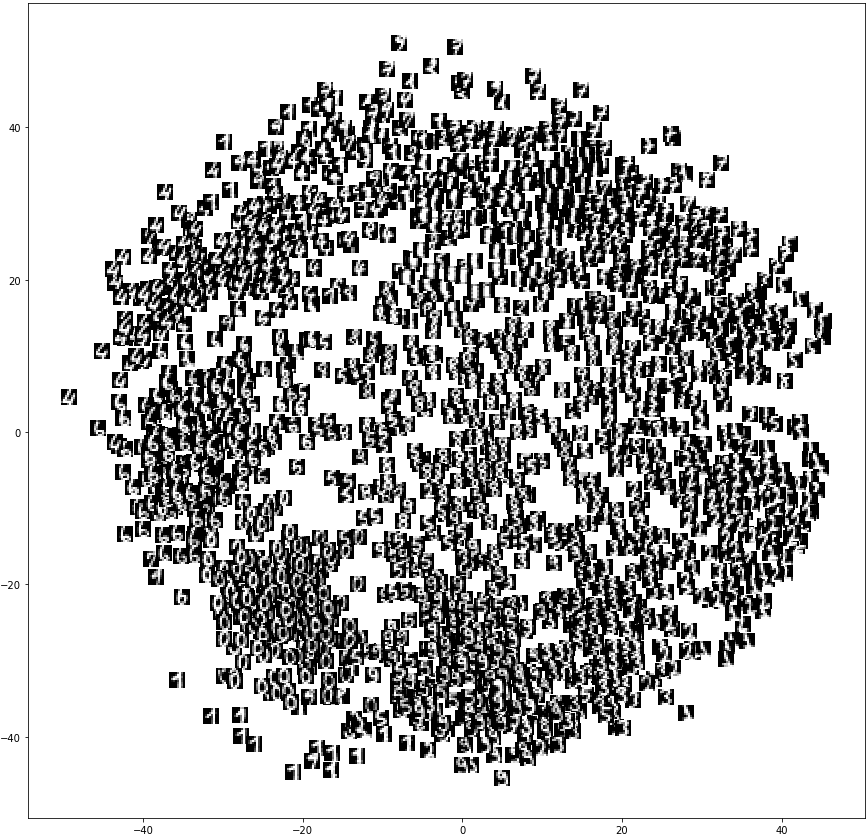
\includegraphics[width=\textwidth]{./figures/mds_2.png}
		\caption{using MDS}
	\end{subfigure}
	\begin{subfigure}[b]{0.4\textwidth}
		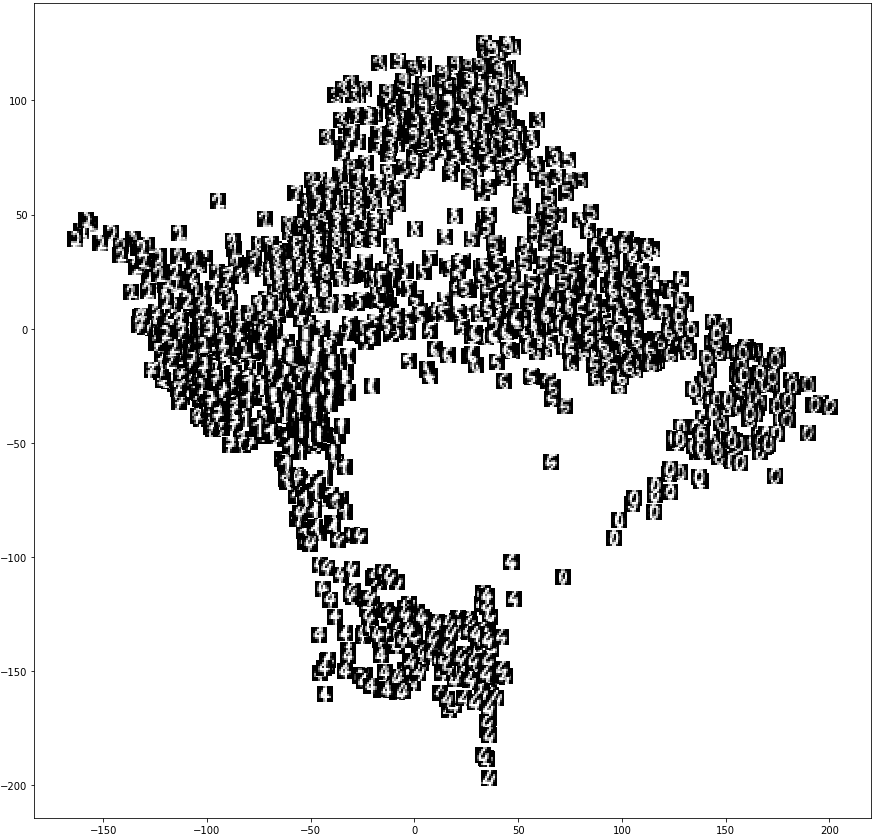
\includegraphics[width=\textwidth]{./figures/isomap_2.png}
		\caption{using Isomap}
	\end{subfigure}
	~
	\begin{subfigure}[b]{0.4\textwidth}
		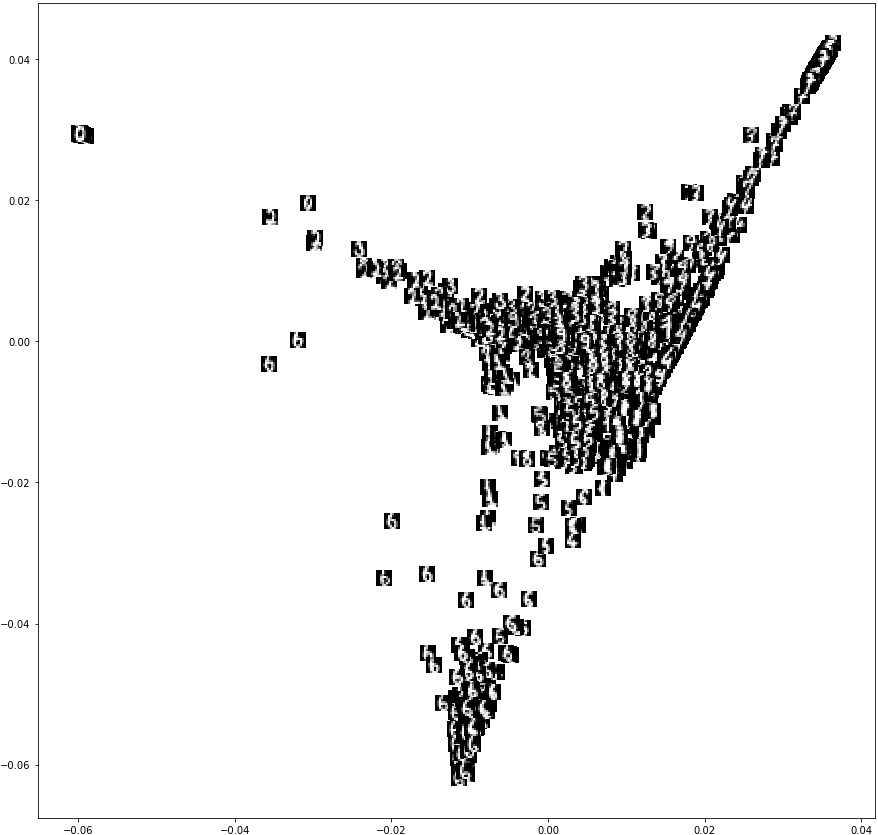
\includegraphics[width=\textwidth]{./figures/lle_2.png}
		\caption{using LLE}
	\end{subfigure}
	
	\begin{subfigure}[b]{0.4\textwidth}
		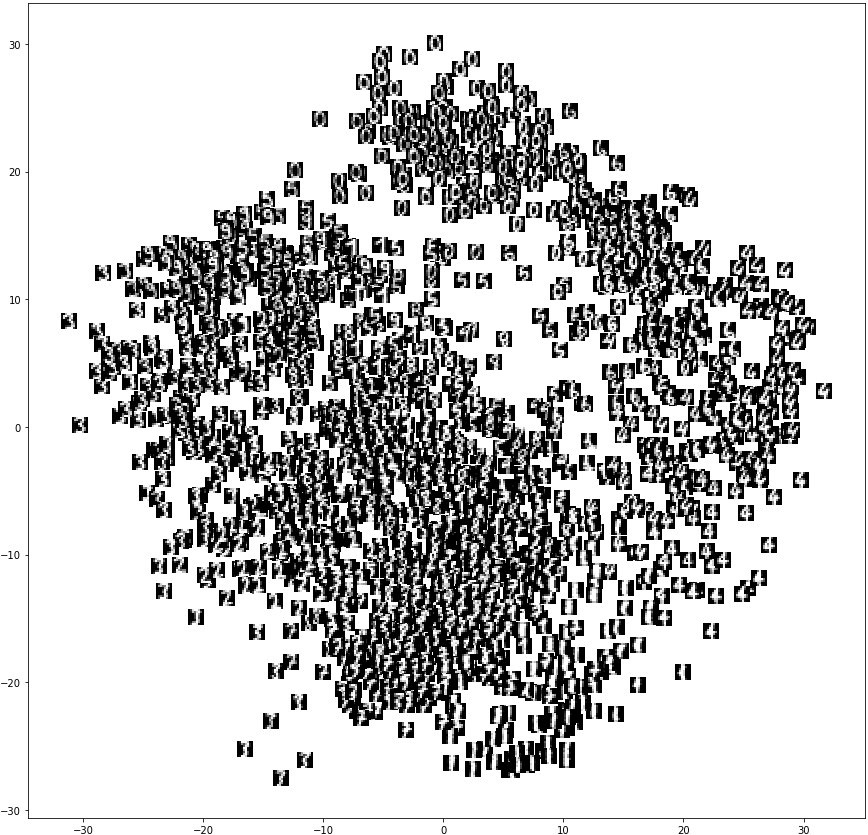
\includegraphics[width=\textwidth]{./figures/pca_2.png}
		\caption{using PCA}
	\end{subfigure}
	~
	\begin{subfigure}[b]{0.4\textwidth}
		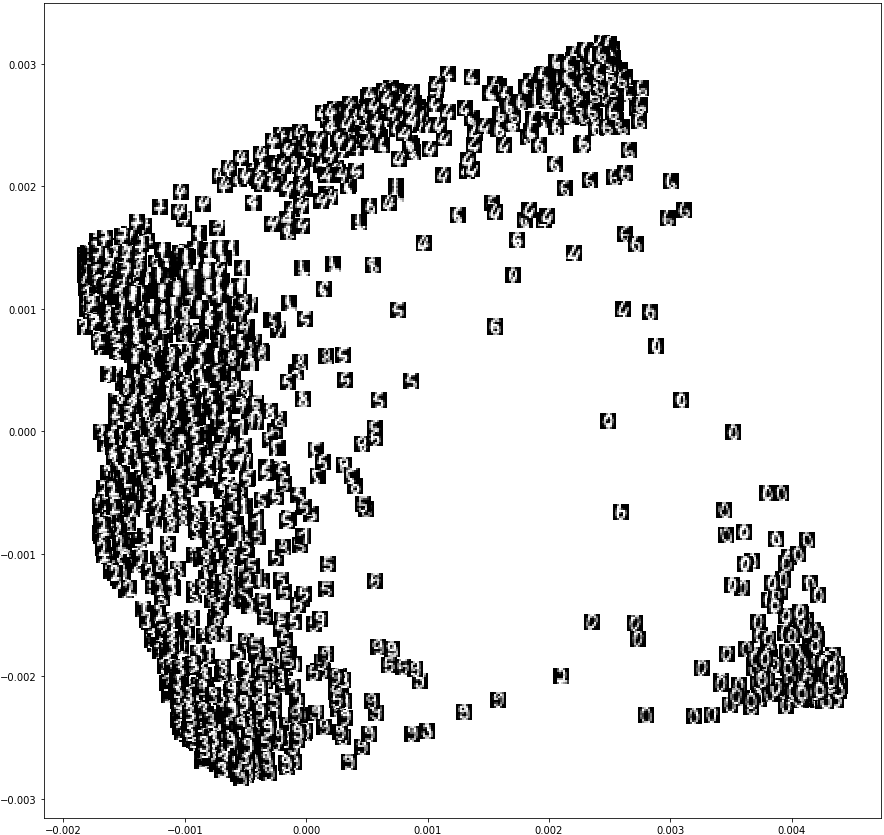
\includegraphics[width=\textwidth]{./figures/lap_2.png}
		\caption{using Laplacian Eigenmaps}
	\end{subfigure}
	
	
	\caption{Visualizations of handwritten digits data set}
\end{figure}



In figures 1-3 we displayed the visualization produced by $t$-SNE, MDS, Isomap, LLE, PCA and Laplacian Eigenmaps algorithms applied to the Olivetti faces data set. Those result support our intuition that $t$-SNE strongly outperforms other techniques in visualization of multidimensional data set. For example, MDS generates ball-like figure, in which only few face classes are visually separated from the other images. Almost all algorithms have few face classes that are correctly clustered and located so that their group is distinct from the others. But at the same they have the majority of images overlapping, which makes it hard to distinguish the borders of the clusters. With such extreme overlaps as in plots produced by LLE or Laplacian Eigenmaps those graphs are almost useless, because if we hadn't class information we would fail to both number of distinct classes and their location. \\

On the contrary, $t$-SNE creates a map with relatively accurate separation of clusters. It locates images of the same person very close to each other, even if some distractions are introduced (like glasses or face rotation). We can observe a number of sole points that don't belong to any cluster. Those are the faces with some specific facial expressions, which $t$-SNE is not able to capture. Besides it, there are some misclassified data points, but most of them correspond to distorted images which is hard to identify.\\

Figure 4 depicts the visualizations obtained after applyting $t$-SNE, MDS, Isomap, LLE, PCA and Laplacian Eigenmaps algorithms to handwritten digits data set. And again, $t$-SNE provides much better visualization capabilities comparing to other visualization techniques. LLE, Laplacian Eigenmaps and Isomap generate some angular structures in which the majority of points are overlapping and borders between classes are not distinguishable. MDS and PCA result in ball-like graphs, in which points of the same class lay close to each other, but in which there is no clear separation between clusters. \\

There is a number points, misclassified by t-SNE algorithm, or such that lay apart from clusters they truly belong to. This can be explained by the relatively small number of features (64), which make instances of different classes look extremely similar.\\

An important quality of any algorithm for visualization of multidimensional data is its speed. Since data analysis in general, and data visualization in particular, is highly iterative process, it is crucial to be able to perform it as fast as possible. The comparison of the visualization techniques in terms of its execution time is given in Table 2.\\

\begin{table}[H]
	\centering
	\begin{tabular}{| l | l | l | l | l | l | l |} 
		\hline
		\quad & $t$-SNE & MDS & Isomap & LLE & PCA & LE \\
		\hline			
		Olivetti faces & \textbf{21.1858} & 3.1424 & 1.2939 & 1.4976 & 0.1158 & 1.2543 \\
		Handwritten digits & \textbf{242.0297} & 73.9359 & 1.7312 & 0.6649 & 0.02638 & 1.5366 \\
		\hline  
	\end{tabular}\\
	\caption{Execution time (in seconds) of discussed visualization algorithms.}
\end{table}

Table 2 demonstrates important weakness of $t$-SNE algorithm - its quadratic computational and memory complexity. This quality makes it impossible to use standard version of this algorithm for data sets that contain more than, for instance, 10000 points. One obvious solution for this problem is to select a random subset of points and display them, but this approach has one serious drawback - we are no longer able to use the information that missing points provide about the underlying manifolds. The way $t$-SNE can be modified in order to use information about the entire data set is well described in the original $t$-SNE paper \cite{tsnearticle}.\\

Another possible solution to this problem is reduce dimensionality of the data set before feeding it into $t$-SNE. This can be performed using PCA, or any other fast dimensionality reduction algorithm.

\subsection{Discussion}

Our experiments showed that $t$-SNE algorithm strongly outperforms other existing techniques for visualization of multidimensional data sets. But still, it has a number of weaknesses, which we would like to discuss deeper.\\

First of all, it's not clear whether $t$-SNE can be used for general dimensionality reduction purposes, when the data is reduced to more than 3 dimentions. The case is, that the heavy tails of Student $t$-distribution do not allow to extrapolate the behavior of this algorithm in 2 or 3 dimensions to higher ones. In high dimensions area under the heavy tails of Student $t$-distribution amounts to a large portion of the probability mass, which might lead to the situation when local structure of the data is not preserved well. \\

Secondly, the cost function of $t$-SNE algorithm is non-convex, which means that several optimization parameters need to be chosen. The solution obtained depend on the optimization parameters choice and may be different each time it is run from the initial random configuration. But in general, it was shown, that even if the optimization process ends up in the local optima, it still provides a visualization good enough to prefer it instead of other visualization techniques. Besides it, the convexity of the cost function can me misleading, because it is often impossible to optimize the function for large data sets, so some appropriate approximation techniques are used instead. \\

The third weakness of $t$-SNE algorithm is its sensitivity to the intristic dimensionality of the data. This can cause the violation of local linearity assumptions on manifold that $t$-SNE makes \cite{tsnearticle}.\\

\section{Conclusions}

\begin{thebibliography}{4}
	\bibitem{tsnearticle} 
	Laurens van der Maaten, Geoffrey Hinton.
	\textit{Visualizing Data using t-SNE}. 
	Journal of Machine Learning Research 9 (2008) 2579-2605
	
	\bibitem{tsnewiki} 
	Wikipedia contributors
	\textit{t-distributed stochastic neighbor embedding}. 
	\\\texttt{https://en.wikipedia.org/wiki/T-distributed\_stochastic\_neighbor\_embedding}
	
	
\end{thebibliography}



\end{document}
